\section{Панель мониторинга}

Для того, чтобы отобразить интегрированные метрики на панель мониторинга, было принято решение использовать
инструмент Graffonet \cite{grafonnet}, который представляет библиотеку на языке Jsonnet \cite{jsonnet}, предназначенную для программной
генерации дашбордов в Grafana \cite{grafana}.

Обычно дашборды в Grafana собирают вручную через интерфейс: кликают, перетаскивают панели, настраивают
фильтры. Но как только графиков становится достаточно много, поддерживать их в актуальном состоянии
превращается в рутинную и затратную работу. Grafonnet решает эту проблему: дашборды
описываются в виде кода, и их можно быстро менять, копировать, хранить в Git и разворачивать
автоматически. Таким образом был изучен язык Jsonnet с фреймворком Grafonnet и были отображены метрики,
представленные в предыдущих пунктах.

На рисунке~\ref{fig:architecture} изображена архитектура сбора метрик. Каждый компонент оснащен одинаковым
HTTP API, который отдает метрики в формате Prometheus по пути \texttt{/metrics}. БД Prometheus собирает
эти метрики с определенным интервалом, который называется \texttt{scrape\_interval}, а затем отдает их в
Grafana, который занимается визуализацией.

\begin{figure}
  \centering
  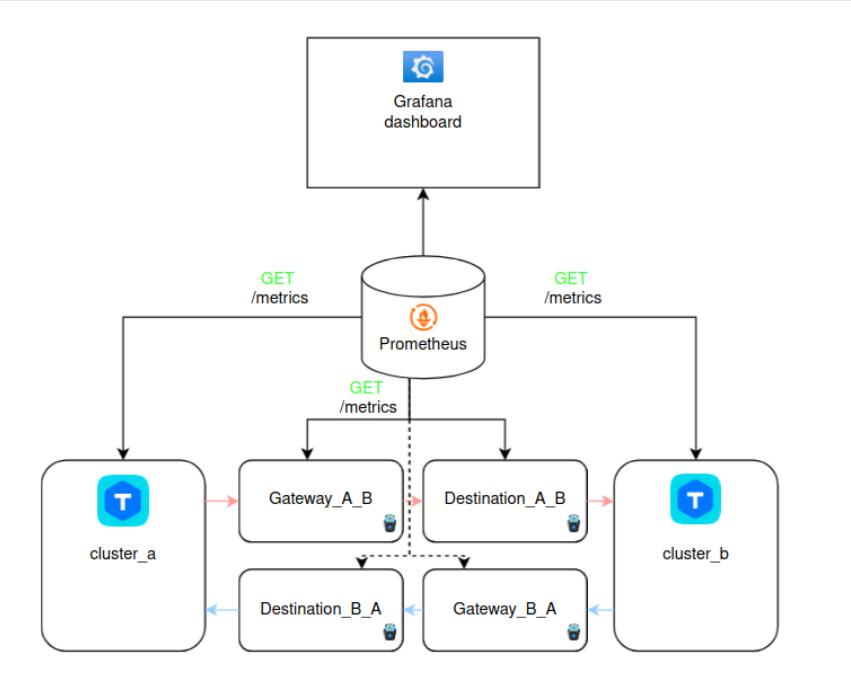
\includegraphics[scale=0.4]{assets/monitoring_architecture.jpg}
  \caption{Архитектура сбора метрик со всех компонентов TCF}
  \label{fig:architecture}
\end{figure}

\subsection{Настройка Prometheus}

Для сбора всех метрик с роли \textit{tcf-worker}, \textit{Gateway}, \textit{Destination} необходимо
написать конфиг с указанием джоб, в котором перечислить все необходимые адреса.

\begin{lstlisting}[frame=rlbt,caption={Пример конфигурации панели мониторинга для Prometheus}]
global:
  scrape_interval: 5s
  evaluation_interval: 5s
 
scrape_configs:
  - job_name: "cluster_a"
    static_configs:
      - targets:
          - localhost:8081
          - localhost:8082
          - localhost:8083
          - localhost:8084
          - localhost:8085
  - job_name: "cluster_b"
    static_configs:
      - targets:
          - localhost:18081
          - localhost:18082
          - localhost:18083
          - localhost:18084
          - localhost:18085
  - job_name: "replicators"
    static_configs:
      - targets:
          - localhost:10081
          - localhost:10082
          - localhost:10181
          - localhost:10182
\end{lstlisting}

Здесь, на листинге 1:

\begin{itemize}
  \item \texttt{scrape\_interval} -- интервал, с которым Prometheus будет собирать метрики (каждые 5 секунд);
  \item \texttt{evaluation\_interval} -- интервал, с которым будет оцениваться состояние правил в Prometheus (5 секунд);
  \item \texttt{scrape\_configs} -- список задач (jobs) для сбора метрик с различных сервисов или кластеров;
  \item \texttt{targets} -- список целей, каждая цель указывает на определённый сервис или экземпляр, с которого Prometheus должен запросить метрики;
  \item \texttt{cluster\_a} -- список адресов сервисов из исходного кластера;
  \item \texttt{cluster\_b} -- список адресов сервисов из целевого кластера;
  \item \texttt{replicators} -- список адресов репликаторов Gateway и Destination.
\end{itemize}

Чтобы правильно отображать метрики репликаторов в Grafana, нужно задать псевдоним (alias) Gateway и
Destination в конфигурации репликаторов данных, в секциях gateway.alias и destination.alias соответственно.

\subsection{Доступные панели и их графики}

В таблице~\ref{tab:metrics} каждой метрике сопоставлены следующие характеристики: панель на дашборде Grafana, а также имя и описание графика.

\begin{longtable}{|>{\raggedright\arraybackslash}p{0.05\textwidth}|
                        >{\raggedright\arraybackslash}p{0.17\textwidth}|
                        >{\raggedright\arraybackslash}p{0.22\textwidth}|
                        >{\raggedright\arraybackslash}p{0.21\textwidth}|
                        >{\raggedright\arraybackslash}p{0.25\textwidth}|}
\caption{Метрики Grafana для репликаторов и кластеров}\label{tab:metrics}\\ \hline
\textbf{№} & \textbf{Панель Grafana} & \textbf{Имя графика} & \textbf{Метрика} & \textbf{Описание графика} \\ \hline
\endfirsthead
\caption*{Продолжение таблицы \ref{tab:metrics}}\\ \hline
\textbf{№} & \textbf{Панель Grafana} & \textbf{Имя графика} & \textbf{Метрика} & \textbf{Описание графика} \\ \hline
\endhead
\hline
\endfoot
\hline
\endlastfoot

1 & Replicators info & Events received from gateway & \metric{tcf_destination_recv_total} &
Общее количество событий, полученных от компонента Gateway \\ \hline

2 & Replicators info & Events read from source cluster & \metric{tcf_gateway_read_total} &
Суммарное количество записей, прочитанных с исходного кластера \\ \hline

3 & Replicators info & Events sent to destination cluster (от gateway) & \metric{tcf_gateway_sent_total} &
Суммарное количество записей, отправленных на компонент Destination \\ \hline

4 & Replicators info & Events sent to destination cluster (or destination) & \metric{tcf_destination_push_total} &
Суммарное количество событий, отправленных в Destination \\ \hline

5 & Replicators info & Vclock signature received from gateway & \metric{tcf_destination_recv_vclock_signature} &
Сигнатура vclock, полученная от компонента Gateway \\ \hline

6 & Replicators info & Vclock signature sent to destination cluster & \metric{tcf_destination_sent_vclock_signature} &
Сигнатура vclock, отправленная из Destination \\ \hline

7 & Replicators info & Vclock signature received from limbo & \metric{tcf_gateway_limbo_vclock_signature} &
Сигнатура vclock из limbo (очереди транзакций) \\ \hline

8 & Replicators info & Vclock signature sent from gateway & \metric{tcf_gateway_sent_vclock_signature} &
Сигнатура vclock, отправленная из Gateway в Destination \\ \hline

9 & Replicators info & Reading from source cluster errors & \metric{tcf_gateway_read_errors_total} &
Суммарное количество ошибок, возникших при чтении данных с исходного кластера \\ \hline

10 & Replicators info & Sending to destination errors & \metric{tcf_gateway_sent_errors_total} &
Суммарное количество ошибок, возникших при отправке данных на компонент Destination \\ \hline

11 & Replicators info & Reading from gateway errors & \metric{tcf_destination_recv_errors_total} &
Общее количество ошибок при получении данных \\ \hline

12 & Replicators info & Sending to destination errors & \metric{tcf_destination_push_errors_total} &
Количество ошибок, возникших в Destination при попытке отправить данные на целевой кластер \\ \hline

13 & Source cluster info / Destination cluster info & Is cluster active & \metric{tcf_is_active} &
Активность текущего кластера: зелёный — активный, жёлтый — пассивный \\ \hline

14 & Source cluster info & Vclock signature sent from source cluster & \metric{tcf_src_vclock_signature} &
Сигнатура vclock, отправленная на Gateway из текущего кластера \\ \hline

15 & Destination cluster info & Vclock signature received from destination cluster & \metric{tcf_dst_vclock_signature} &
Сигнатура vclock, применённая на целевом кластере \\ \hline

\end{longtable}

На рисунке~\ref{fig:fig02} представлены графики №1-4 из таблицы~\ref{tab:metrics}. Все 4 графика повторяют
друг друга, что означает отсутствие потерь на каждом из репликаторов при репликации данных.

\begin{figure}
  \centering
  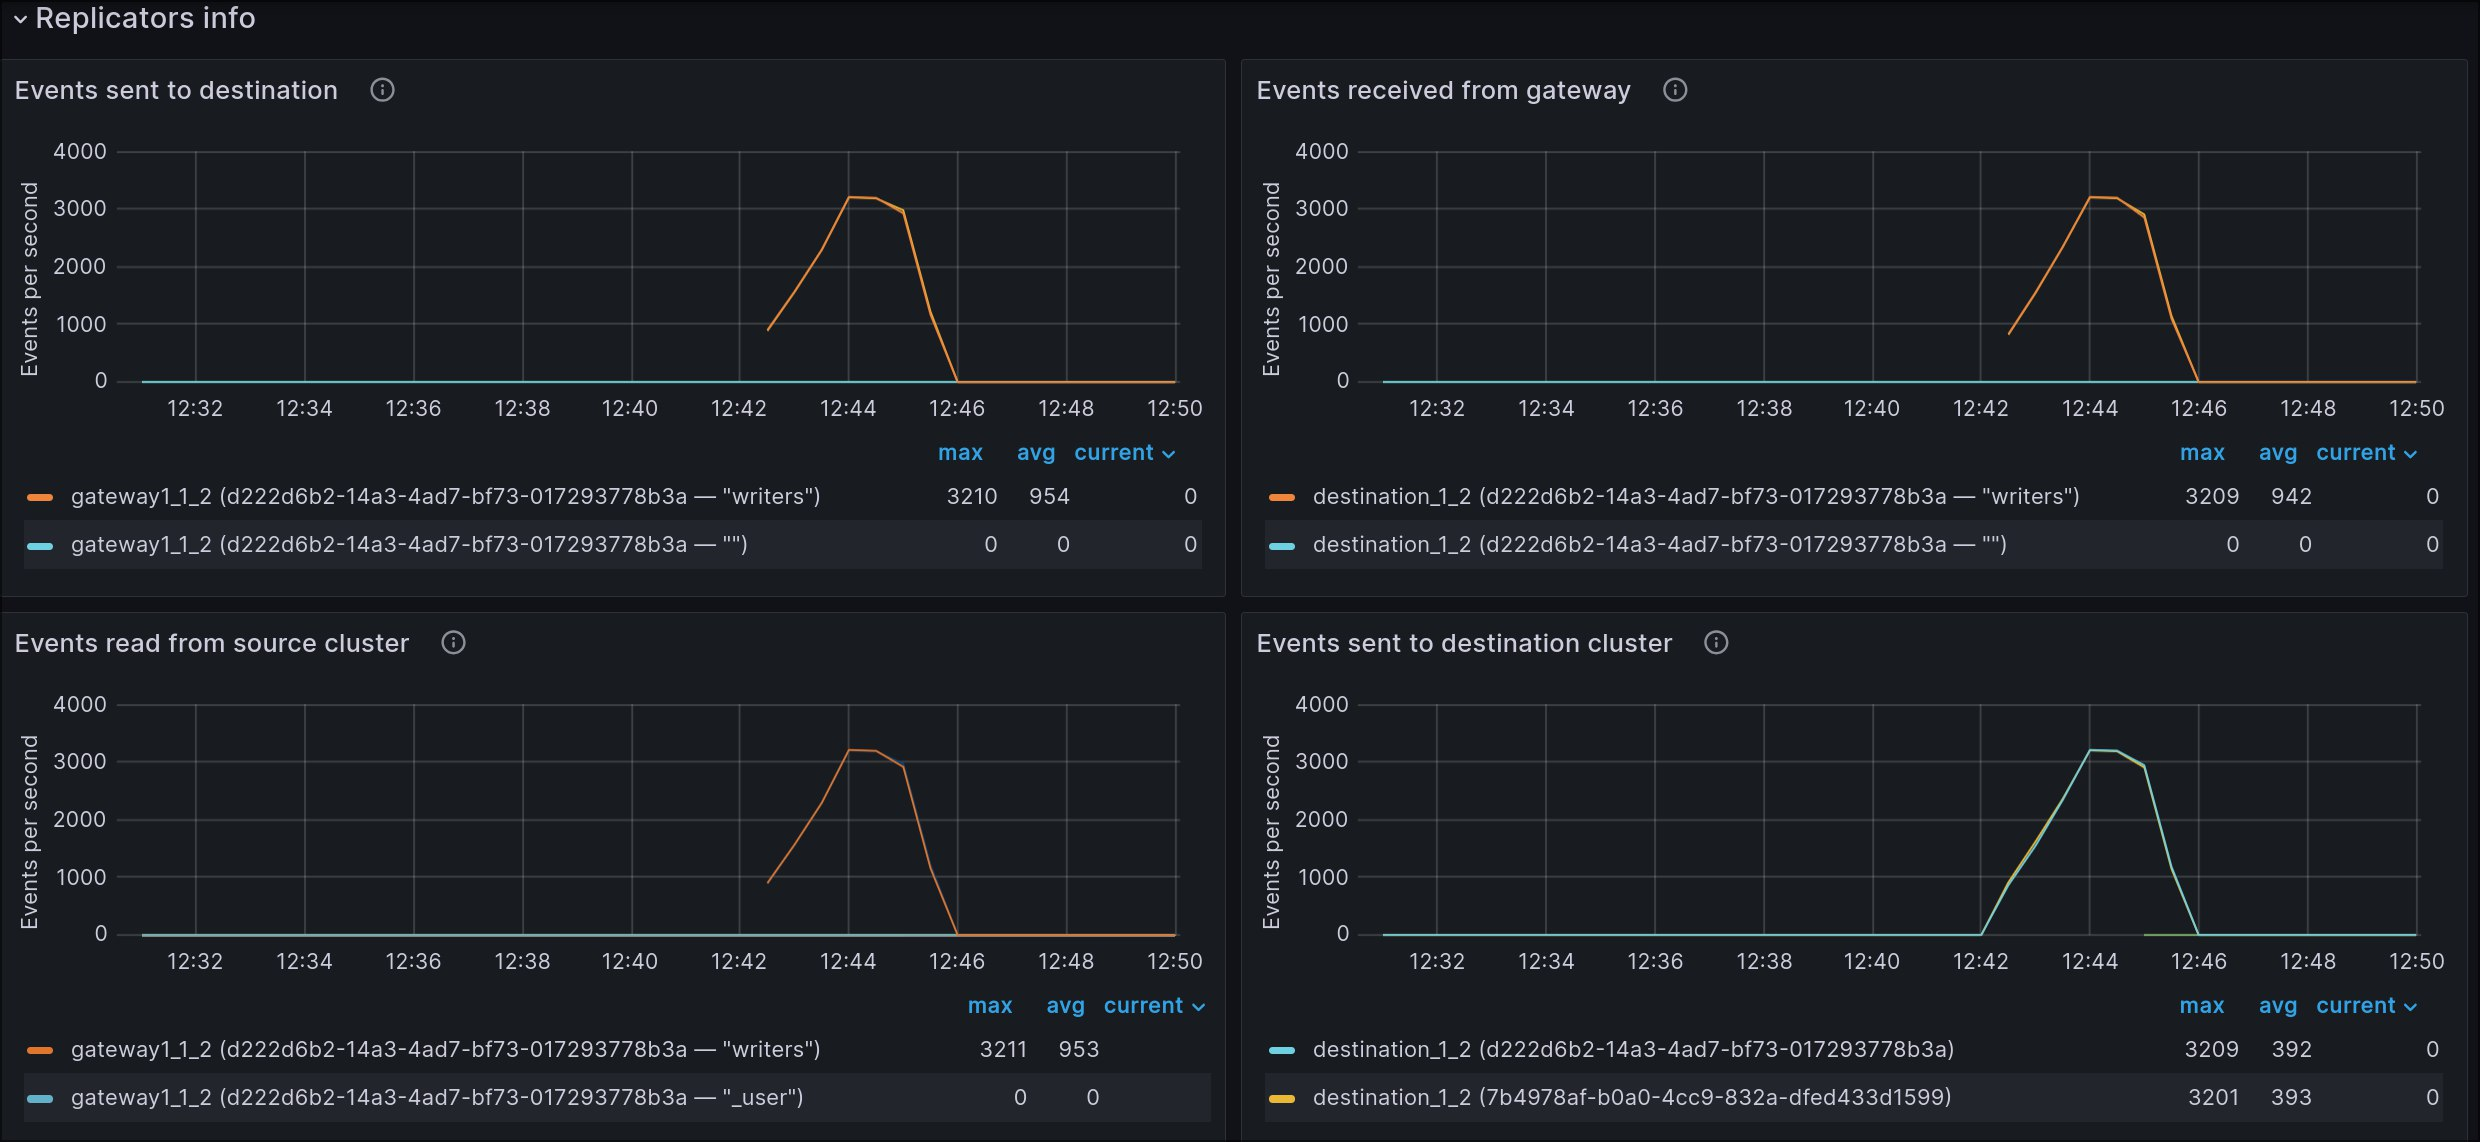
\includegraphics[scale=0.2]{assets/replicators_info_graph_1.jpeg}
  \caption{Графики репликаторов с количеством обработанных событий в секунду}
  \label{fig:fig02}
\end{figure}

На рисунке~\ref{fig:fig03} представлены графики №5-8 из таблицы~\ref{tab:metrics}. Как видно из одинаковых
графиков, сигнатуры повторяются, что явяляется штатной ситуацией.

\begin{figure}
  \centering
  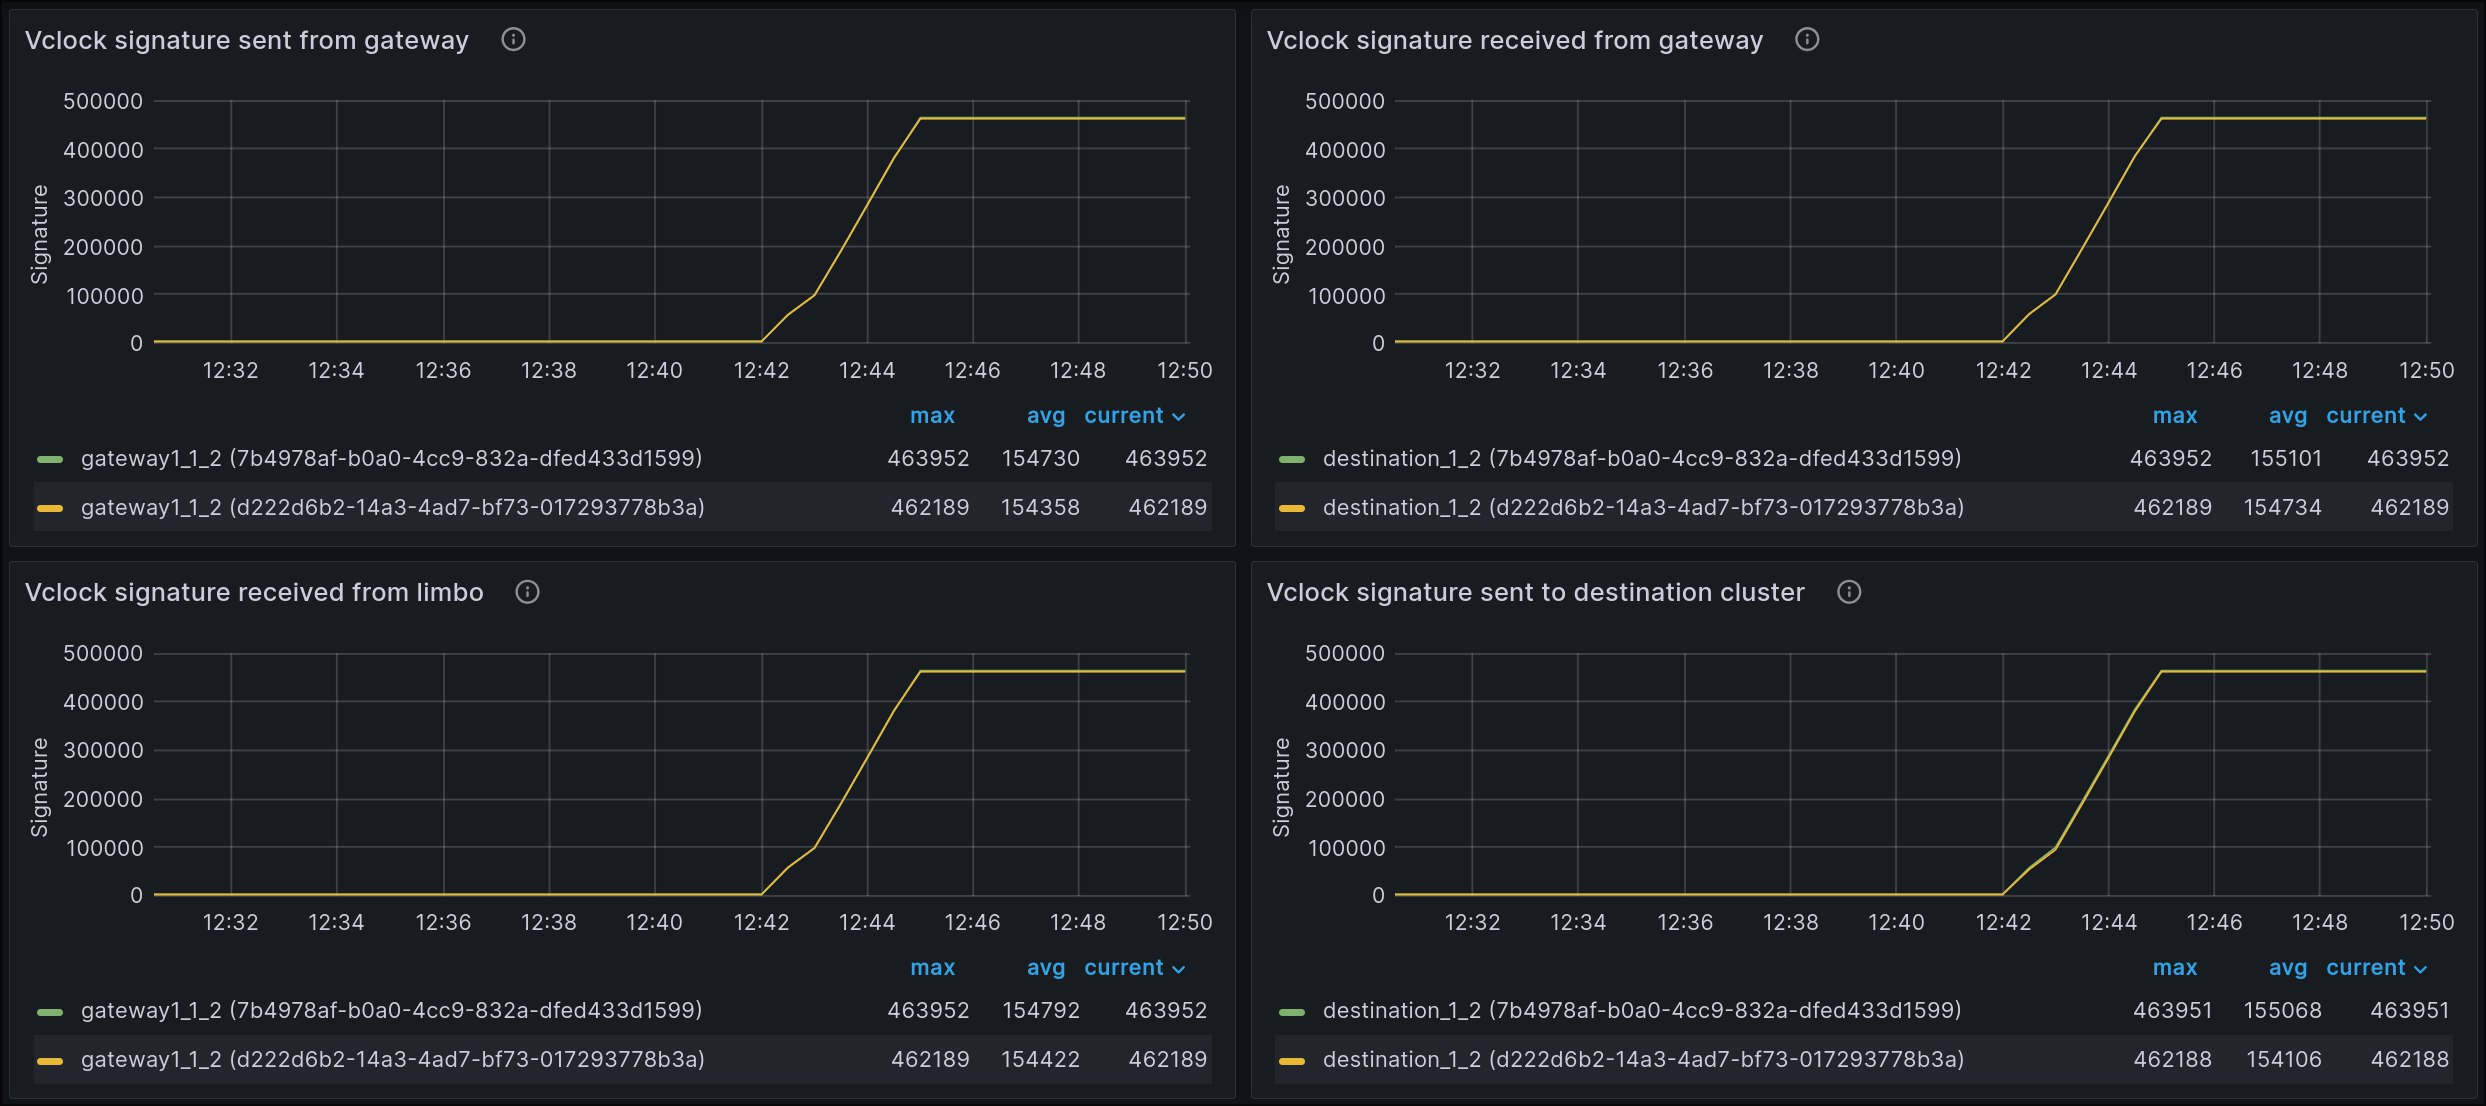
\includegraphics[scale=0.2]{assets/replicators_info_graph_2.jpeg}
  \caption{Графики репликаторов с сигнатурой векторных часов на каждом этапе}
  \label{fig:fig03}
\end{figure}

На рисунке~\ref{fig:fig04} представлены графики №9-12 из таблицы~\ref{tab:metrics}. На графиках ошибок
наблюдается только одна, что говорит о закрытии репликационного потока. Так как запрос на репликацию
повторился, поток переоткрылся, а значит ситуация не является аварийной. На графиках RPS HTTP-запросов
видны запрос на старт \textit{Gateway} и получение статуса \textit{Destination}.

\begin{figure}
  \centering
  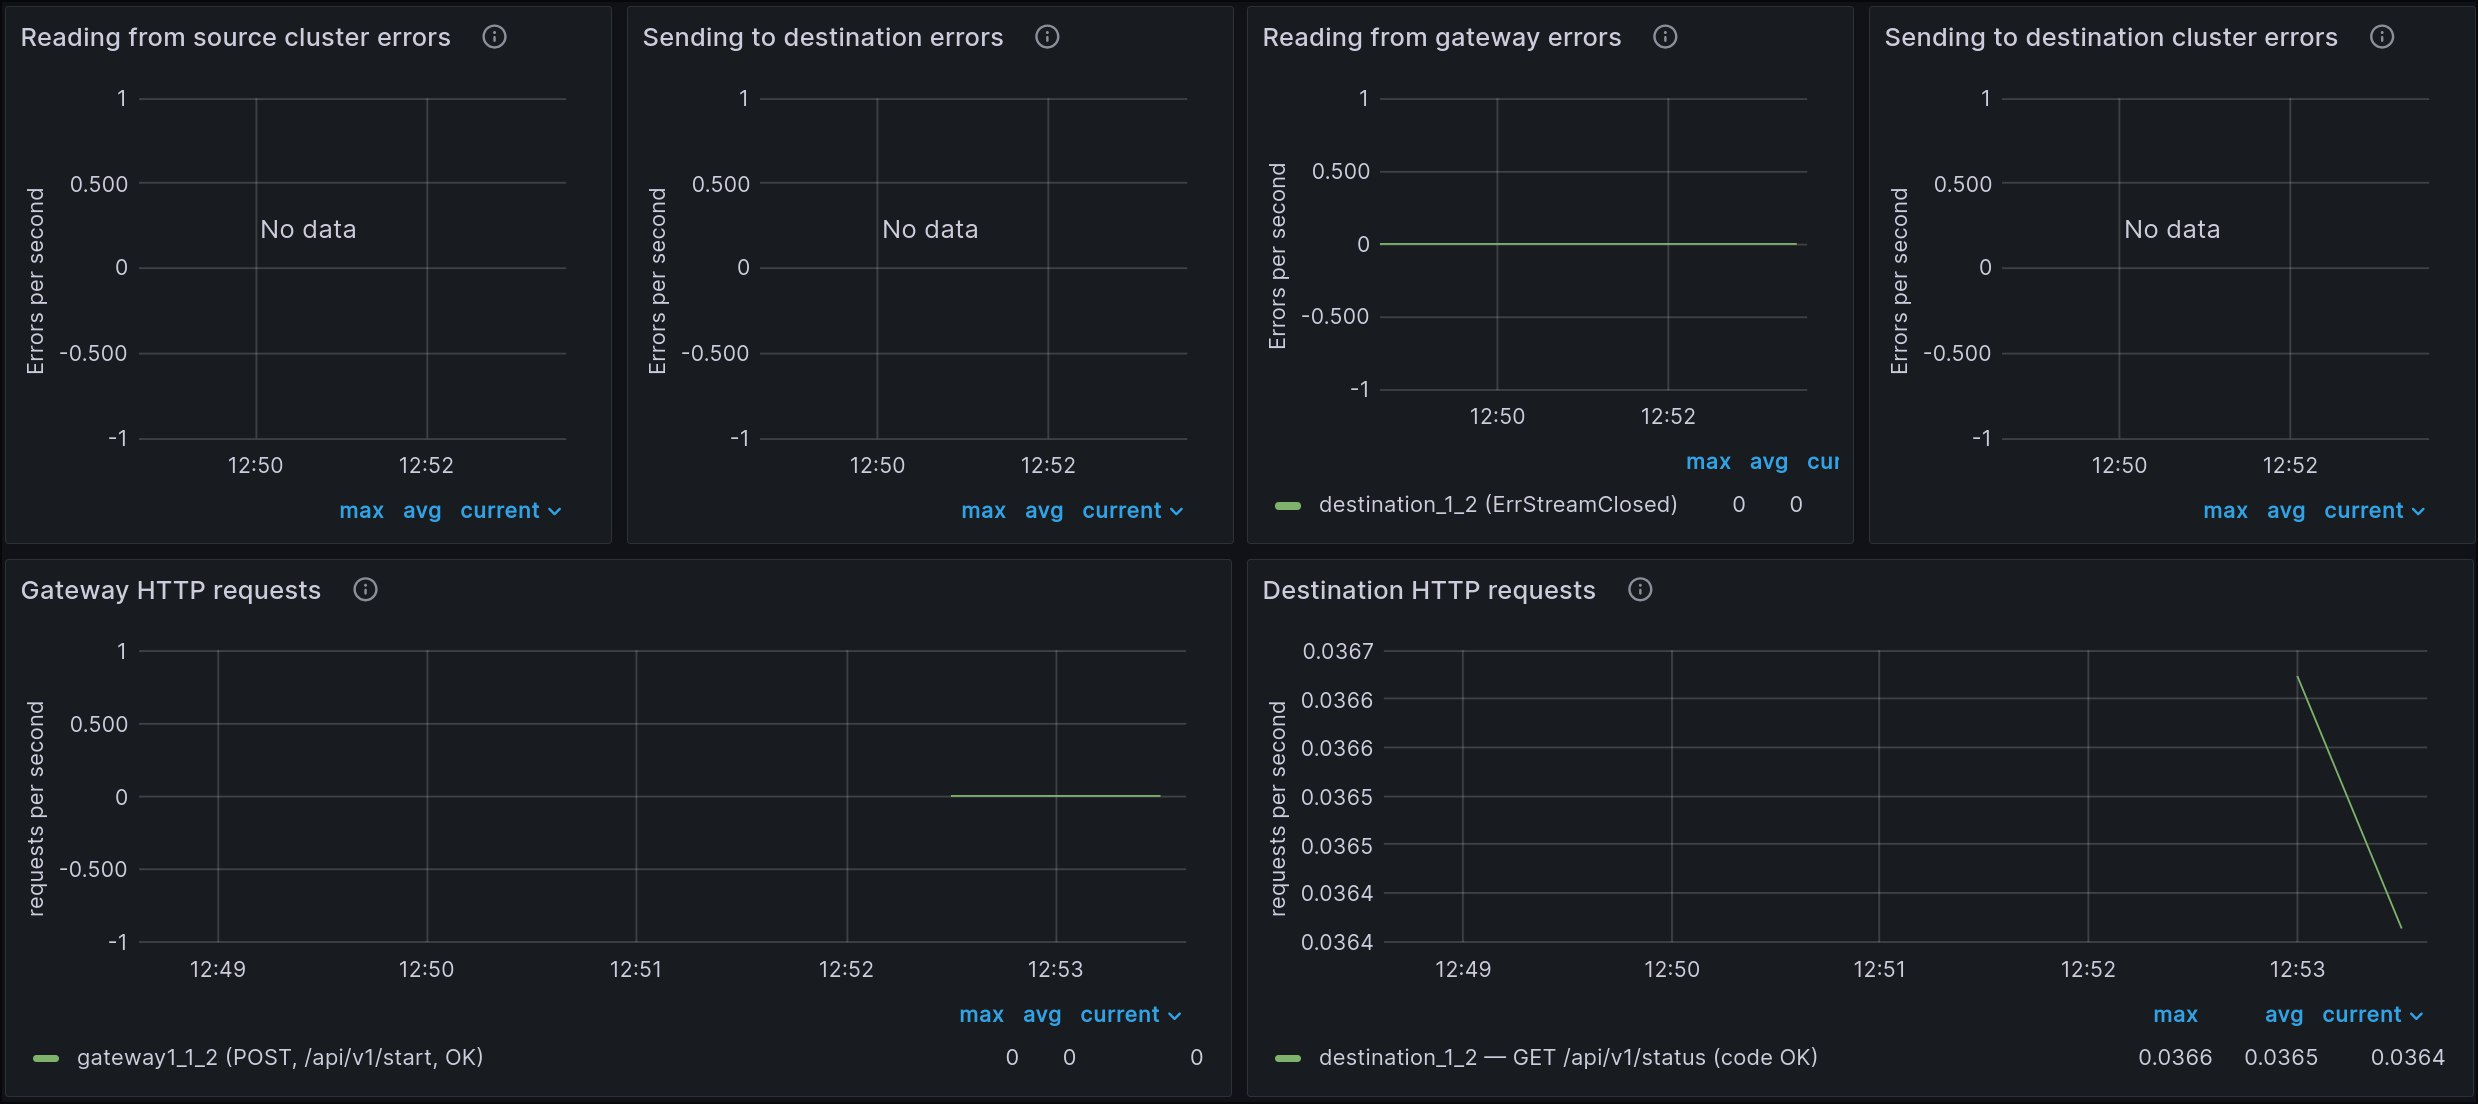
\includegraphics[scale=0.2]{assets/replicators_info_graph_3.jpeg}
  \caption{Графики репликаторов с отображением ошибок и статусами HTTP-запросов}
  \label{fig:fig04}
\end{figure}

На рисунке~\ref{fig:fig05} представлена панель №14 из таблицы~\ref{tab:metrics}. На графиках виден активный
статус кластера, растущую сигнатуру, говорящую о реплицируемых данных. Также виден пустой график сигнатуры
соседнего кластера, так как репликации в обратную сторону еще не было. HTTP-запросы на этот кластер не
поступали, поэтому последний график пуст.

\begin{figure}
  \centering
  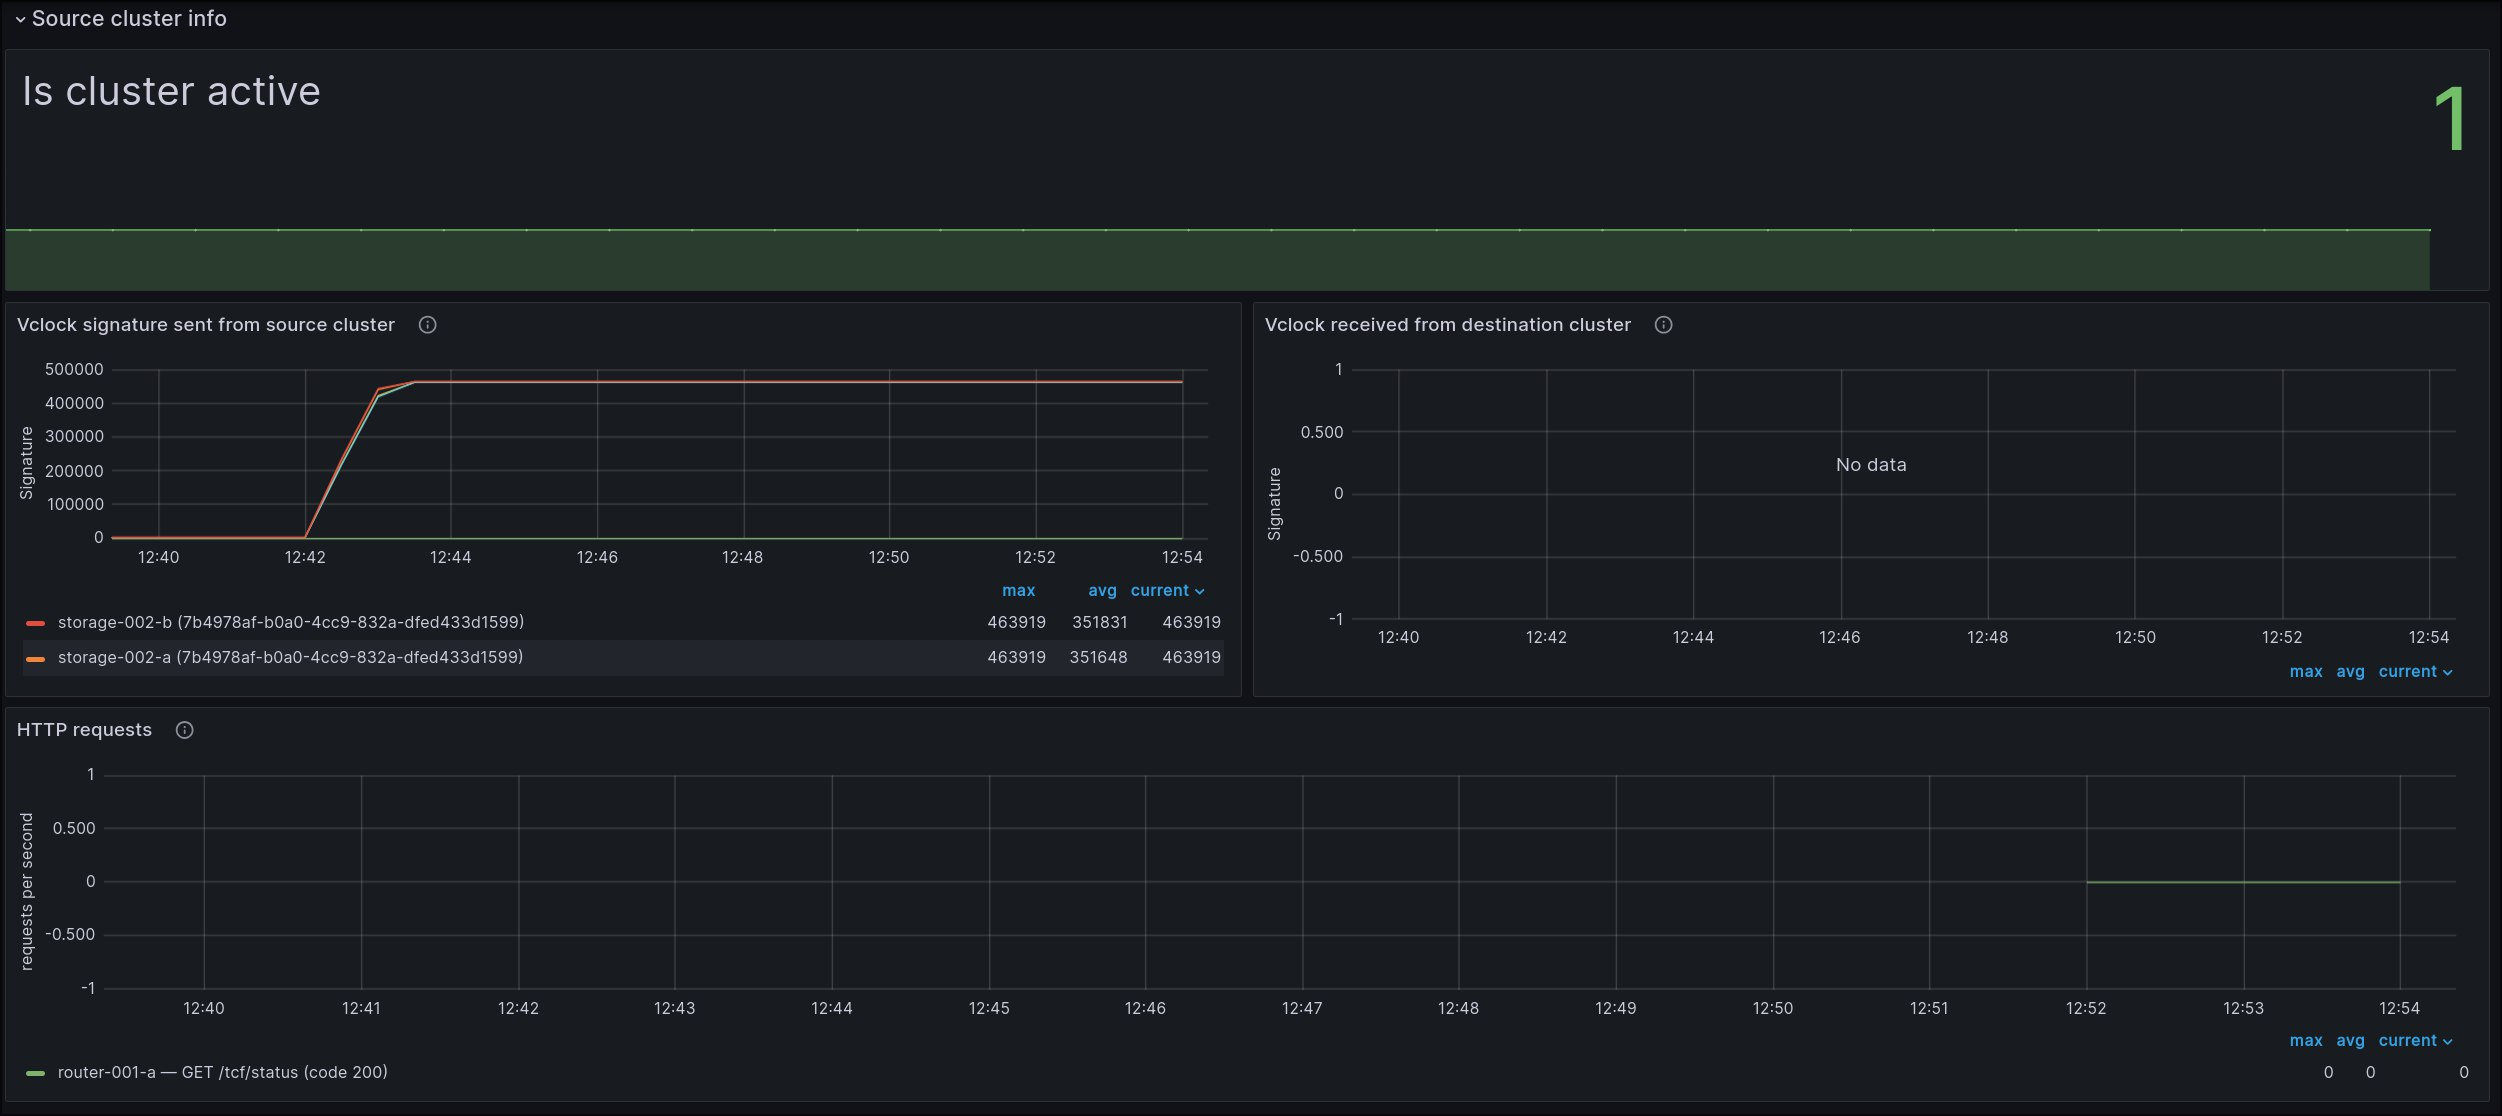
\includegraphics[scale=0.2]{assets/source_cluster_info.jpeg}
  \caption{Панель кластера-источника}
  \label{fig:fig05}
\end{figure}

На рисунке~\ref{fig:fig06} представлена панель №15 из таблицы~\ref{tab:metrics}. На графиках виден
пассивный статус кластера, растущую сигнатуру, говорящую о реплицируемых данных. Здесь график соседнего
не пустой, так как с него идет нагрузка. На этот кластер HTTP-запросов также не поступало.

\begin{figure}
  \centering
  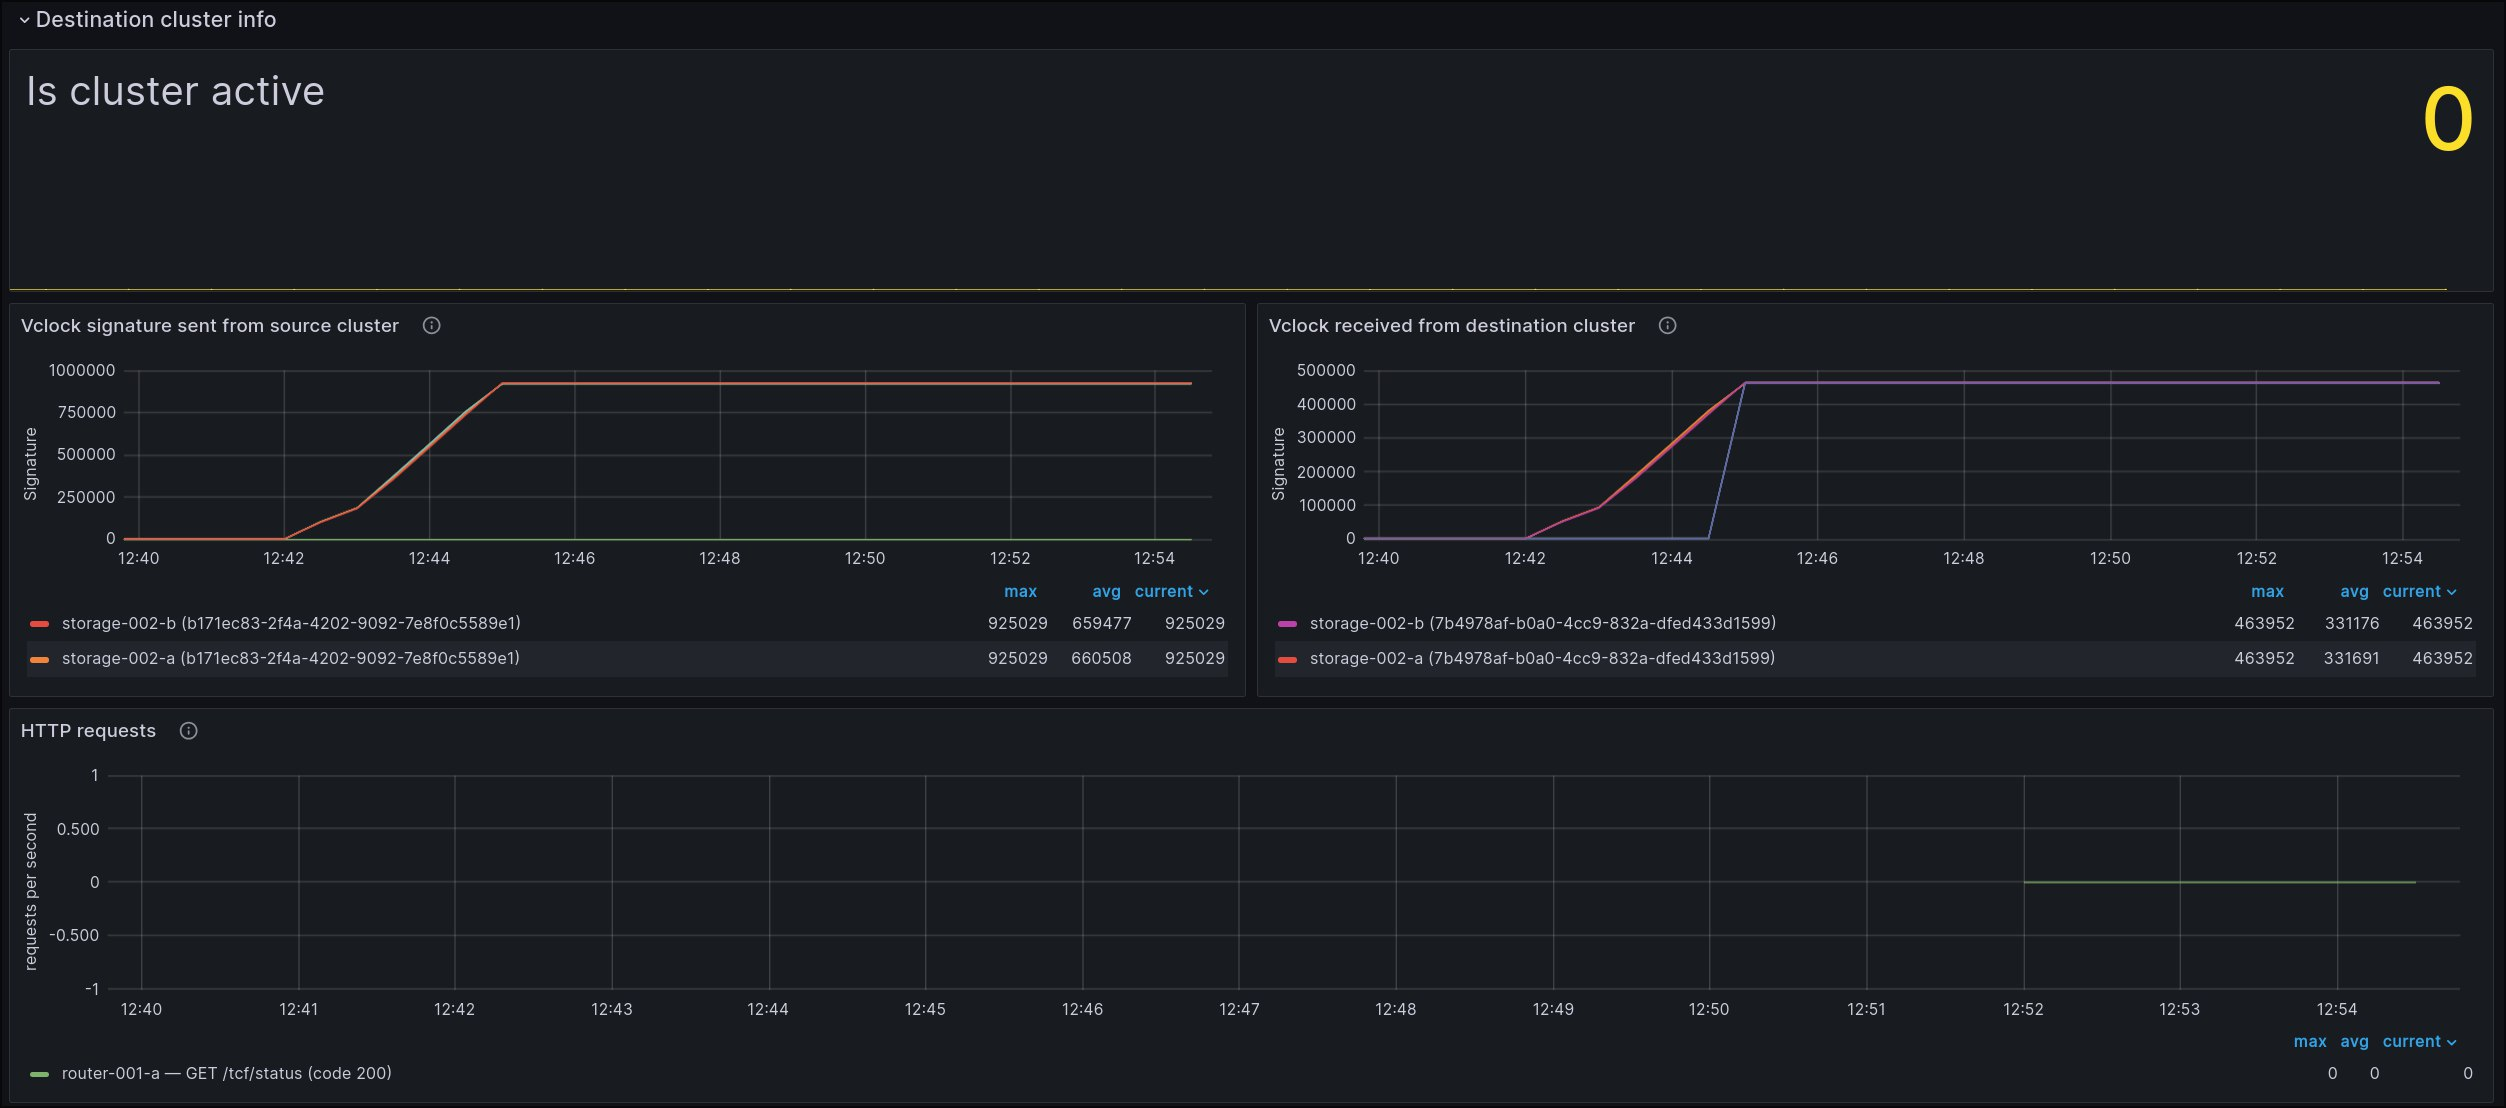
\includegraphics[scale=0.2]{assets/destination_cluster_info.jpeg}
  \caption{Панель кластера назначения}
  \label{fig:fig06}
\end{figure}

На рисунке~\ref{fig:fig07} представлены графики системных метрик репликаторов: количество выделенных
горутин, использованной памяти, выделение, освобождение памяти и т. д.

\begin{figure}
  \centering
  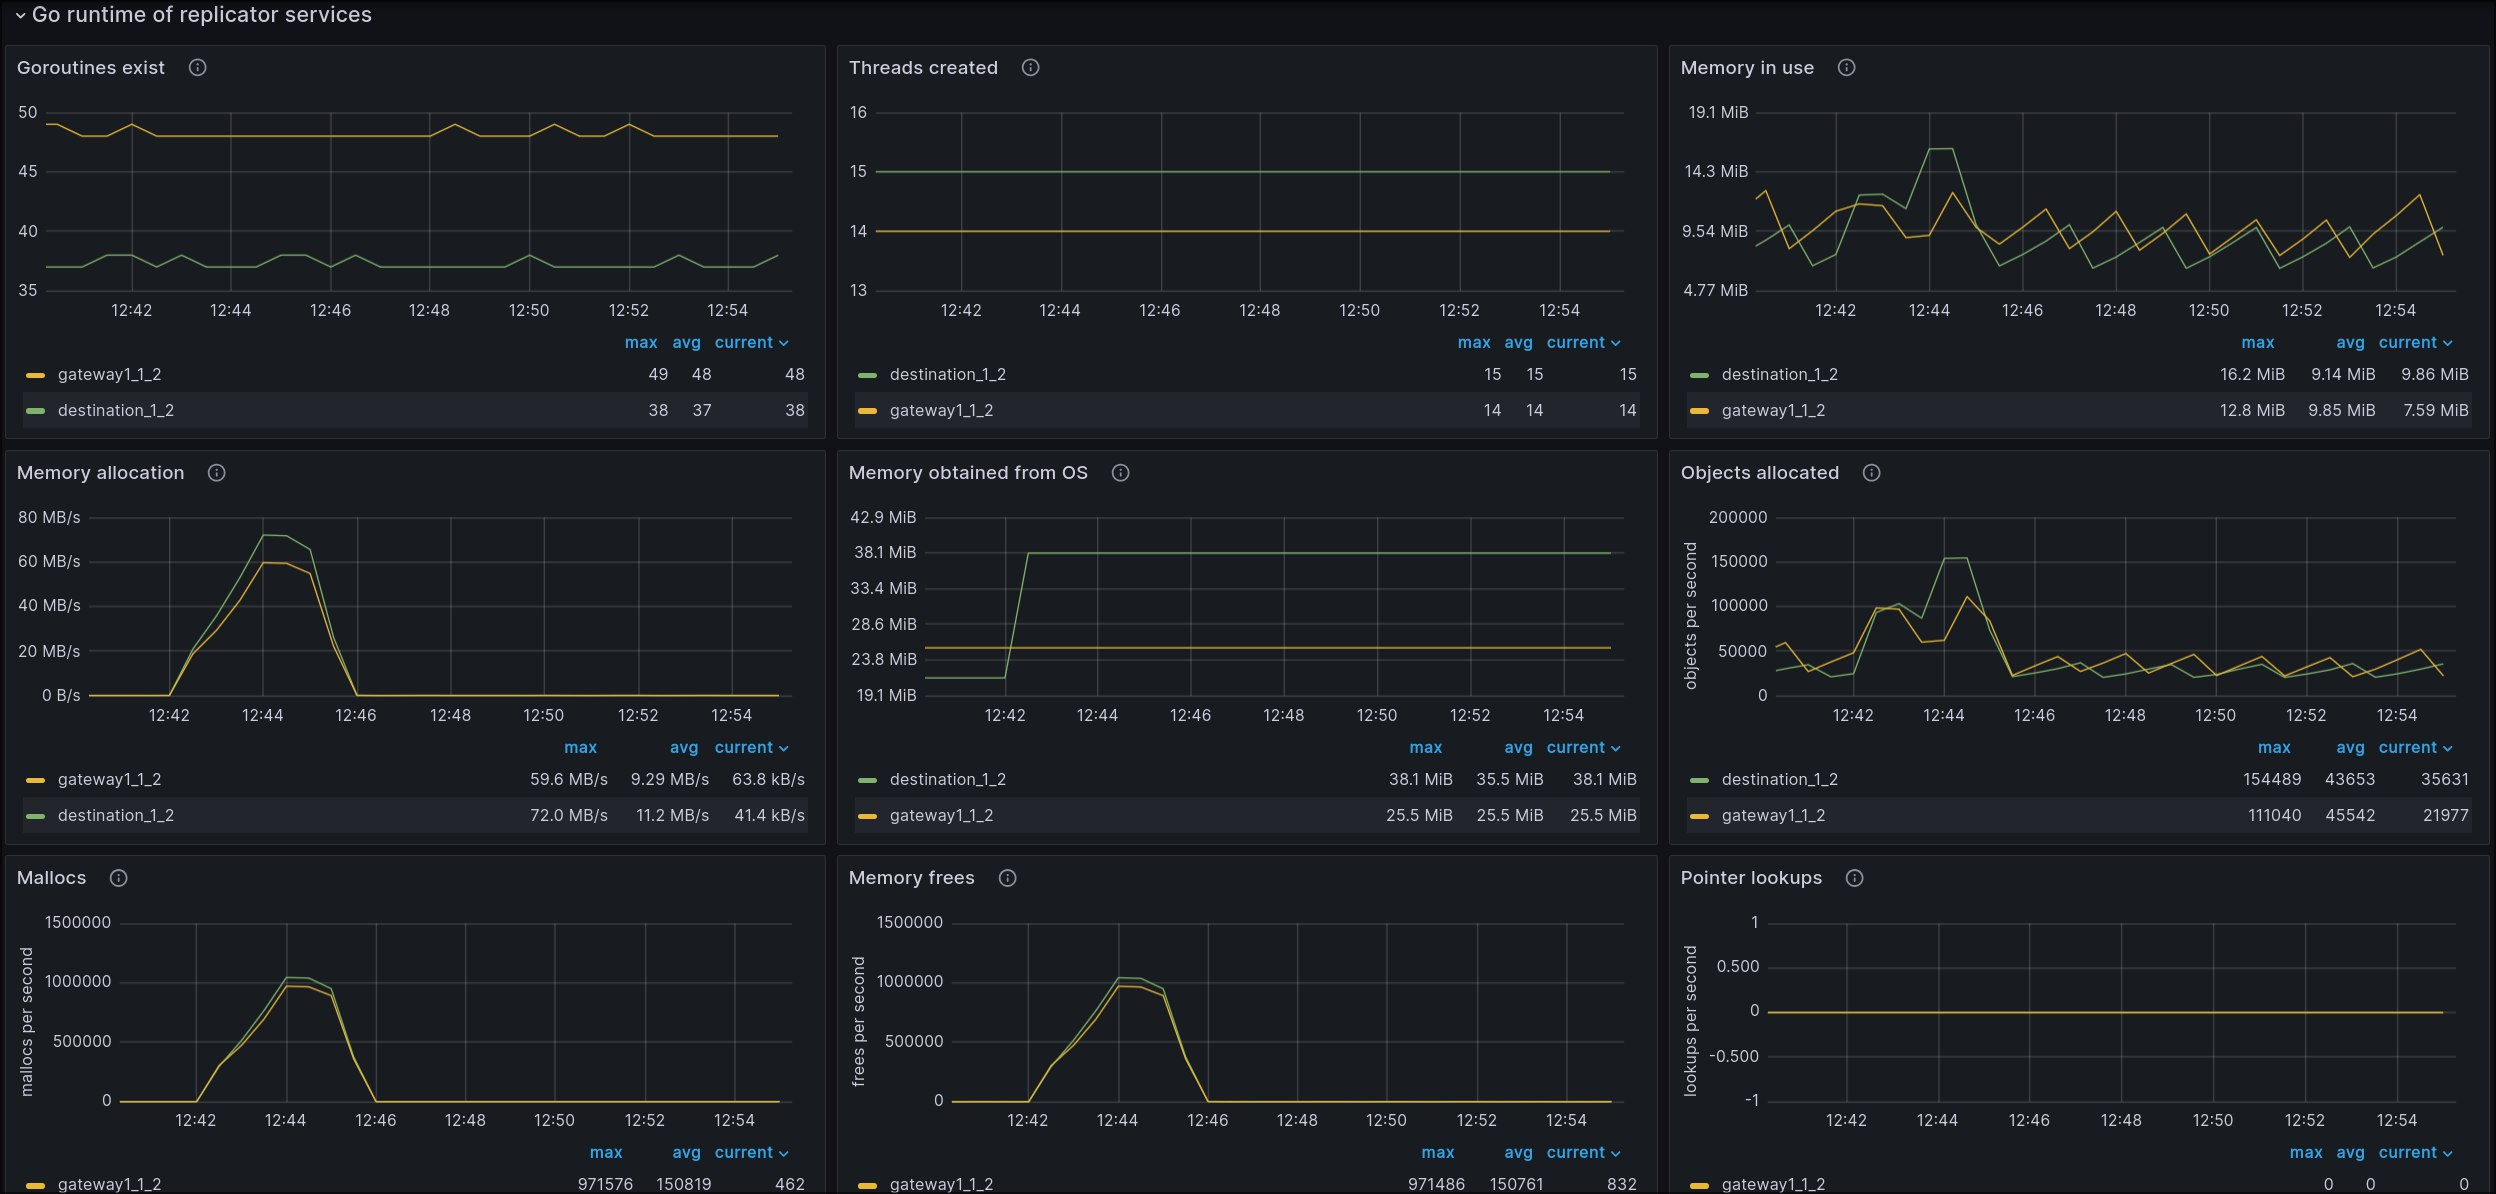
\includegraphics[scale=0.2]{assets/go_runtime_graph.jpeg}
  \caption{Панель системных метрик репликаторов}
  \label{fig:fig07}
\end{figure}
